% Options for packages loaded elsewhere
\PassOptionsToPackage{unicode}{hyperref}
\PassOptionsToPackage{hyphens}{url}
\PassOptionsToPackage{dvipsnames,svgnames,x11names}{xcolor}
%
\documentclass[
  10pt,
  letterpaper]{article}

\usepackage{amsmath,amssymb}
\usepackage{lmodern}
\usepackage{iftex}
\ifPDFTeX
  \usepackage[T1]{fontenc}
  \usepackage[utf8]{inputenc}
  \usepackage{textcomp} % provide euro and other symbols
\else % if luatex or xetex
  \usepackage{unicode-math}
  \defaultfontfeatures{Scale=MatchLowercase}
  \defaultfontfeatures[\rmfamily]{Ligatures=TeX,Scale=1}
  \setmainfont[]{Charis SIL}
  \setmonofont[]{Monaco}
  \setmathfont[]{Monaco}
\fi
% Use upquote if available, for straight quotes in verbatim environments
\IfFileExists{upquote.sty}{\usepackage{upquote}}{}
\IfFileExists{microtype.sty}{% use microtype if available
  \usepackage[]{microtype}
  \UseMicrotypeSet[protrusion]{basicmath} % disable protrusion for tt fonts
}{}
\makeatletter
\@ifundefined{KOMAClassName}{% if non-KOMA class
  \IfFileExists{parskip.sty}{%
    \usepackage{parskip}
  }{% else
    \setlength{\parindent}{0pt}
    \setlength{\parskip}{6pt plus 2pt minus 1pt}}
}{% if KOMA class
  \KOMAoptions{parskip=half}}
\makeatother
\usepackage{xcolor}
\usepackage[margin = 1in]{geometry}
\setlength{\emergencystretch}{3em} % prevent overfull lines
\setcounter{secnumdepth}{-\maxdimen} % remove section numbering
% Make \paragraph and \subparagraph free-standing
\ifx\paragraph\undefined\else
  \let\oldparagraph\paragraph
  \renewcommand{\paragraph}[1]{\oldparagraph{#1}\mbox{}}
\fi
\ifx\subparagraph\undefined\else
  \let\oldsubparagraph\subparagraph
  \renewcommand{\subparagraph}[1]{\oldsubparagraph{#1}\mbox{}}
\fi

\usepackage{color}
\usepackage{fancyvrb}
\newcommand{\VerbBar}{|}
\newcommand{\VERB}{\Verb[commandchars=\\\{\}]}
\DefineVerbatimEnvironment{Highlighting}{Verbatim}{commandchars=\\\{\}}
% Add ',fontsize=\small' for more characters per line
\usepackage{framed}
\definecolor{shadecolor}{RGB}{241,243,245}
\newenvironment{Shaded}{\begin{snugshade}}{\end{snugshade}}
\newcommand{\AlertTok}[1]{\textcolor[rgb]{0.68,0.00,0.00}{#1}}
\newcommand{\AnnotationTok}[1]{\textcolor[rgb]{0.37,0.37,0.37}{#1}}
\newcommand{\AttributeTok}[1]{\textcolor[rgb]{0.40,0.45,0.13}{#1}}
\newcommand{\BaseNTok}[1]{\textcolor[rgb]{0.68,0.00,0.00}{#1}}
\newcommand{\BuiltInTok}[1]{\textcolor[rgb]{0.00,0.23,0.31}{#1}}
\newcommand{\CharTok}[1]{\textcolor[rgb]{0.13,0.47,0.30}{#1}}
\newcommand{\CommentTok}[1]{\textcolor[rgb]{0.37,0.37,0.37}{#1}}
\newcommand{\CommentVarTok}[1]{\textcolor[rgb]{0.37,0.37,0.37}{\textit{#1}}}
\newcommand{\ConstantTok}[1]{\textcolor[rgb]{0.56,0.35,0.01}{#1}}
\newcommand{\ControlFlowTok}[1]{\textcolor[rgb]{0.00,0.23,0.31}{#1}}
\newcommand{\DataTypeTok}[1]{\textcolor[rgb]{0.68,0.00,0.00}{#1}}
\newcommand{\DecValTok}[1]{\textcolor[rgb]{0.68,0.00,0.00}{#1}}
\newcommand{\DocumentationTok}[1]{\textcolor[rgb]{0.37,0.37,0.37}{\textit{#1}}}
\newcommand{\ErrorTok}[1]{\textcolor[rgb]{0.68,0.00,0.00}{#1}}
\newcommand{\ExtensionTok}[1]{\textcolor[rgb]{0.00,0.23,0.31}{#1}}
\newcommand{\FloatTok}[1]{\textcolor[rgb]{0.68,0.00,0.00}{#1}}
\newcommand{\FunctionTok}[1]{\textcolor[rgb]{0.28,0.35,0.67}{#1}}
\newcommand{\ImportTok}[1]{\textcolor[rgb]{0.00,0.46,0.62}{#1}}
\newcommand{\InformationTok}[1]{\textcolor[rgb]{0.37,0.37,0.37}{#1}}
\newcommand{\KeywordTok}[1]{\textcolor[rgb]{0.00,0.23,0.31}{#1}}
\newcommand{\NormalTok}[1]{\textcolor[rgb]{0.00,0.23,0.31}{#1}}
\newcommand{\OperatorTok}[1]{\textcolor[rgb]{0.37,0.37,0.37}{#1}}
\newcommand{\OtherTok}[1]{\textcolor[rgb]{0.00,0.23,0.31}{#1}}
\newcommand{\PreprocessorTok}[1]{\textcolor[rgb]{0.68,0.00,0.00}{#1}}
\newcommand{\RegionMarkerTok}[1]{\textcolor[rgb]{0.00,0.23,0.31}{#1}}
\newcommand{\SpecialCharTok}[1]{\textcolor[rgb]{0.37,0.37,0.37}{#1}}
\newcommand{\SpecialStringTok}[1]{\textcolor[rgb]{0.13,0.47,0.30}{#1}}
\newcommand{\StringTok}[1]{\textcolor[rgb]{0.13,0.47,0.30}{#1}}
\newcommand{\VariableTok}[1]{\textcolor[rgb]{0.07,0.07,0.07}{#1}}
\newcommand{\VerbatimStringTok}[1]{\textcolor[rgb]{0.13,0.47,0.30}{#1}}
\newcommand{\WarningTok}[1]{\textcolor[rgb]{0.37,0.37,0.37}{\textit{#1}}}

\providecommand{\tightlist}{%
  \setlength{\itemsep}{0pt}\setlength{\parskip}{0pt}}\usepackage{longtable,booktabs,array}
\usepackage{calc} % for calculating minipage widths
% Correct order of tables after \paragraph or \subparagraph
\usepackage{etoolbox}
\makeatletter
\patchcmd\longtable{\par}{\if@noskipsec\mbox{}\fi\par}{}{}
\makeatother
% Allow footnotes in longtable head/foot
\IfFileExists{footnotehyper.sty}{\usepackage{footnotehyper}}{\usepackage{footnote}}
\makesavenoteenv{longtable}
\usepackage{graphicx}
\makeatletter
\def\maxwidth{\ifdim\Gin@nat@width>\linewidth\linewidth\else\Gin@nat@width\fi}
\def\maxheight{\ifdim\Gin@nat@height>\textheight\textheight\else\Gin@nat@height\fi}
\makeatother
% Scale images if necessary, so that they will not overflow the page
% margins by default, and it is still possible to overwrite the defaults
% using explicit options in \includegraphics[width, height, ...]{}
\setkeys{Gin}{width=\maxwidth,height=\maxheight,keepaspectratio}
% Set default figure placement to htbp
\makeatletter
\def\fps@figure{htbp}
\makeatother

\usepackage{tabularx}
\usepackage{threeparttable}
\usepackage{booktabs}
\usepackage{tipa}
\let\Oldtexttt\texttt
\renewcommand\texttt[1]{{\ttfamily\color{BrickRed}#1}}
\usepackage{authoraftertitle}
\usepackage{fancyhdr}
\pagestyle{fancy}
\rfoot{\copyright Matt Hunt Gardner}
\cfoot{\thepage}
\lhead{Doing LVC with \textit{R}: \MyTitle}
\rhead{}
\makeatletter
\@ifpackageloaded{tcolorbox}{}{\usepackage[many]{tcolorbox}}
\@ifpackageloaded{fontawesome5}{}{\usepackage{fontawesome5}}
\definecolor{quarto-callout-color}{HTML}{909090}
\definecolor{quarto-callout-note-color}{HTML}{0758E5}
\definecolor{quarto-callout-important-color}{HTML}{CC1914}
\definecolor{quarto-callout-warning-color}{HTML}{EB9113}
\definecolor{quarto-callout-tip-color}{HTML}{00A047}
\definecolor{quarto-callout-caution-color}{HTML}{FC5300}
\definecolor{quarto-callout-color-frame}{HTML}{acacac}
\definecolor{quarto-callout-note-color-frame}{HTML}{4582ec}
\definecolor{quarto-callout-important-color-frame}{HTML}{d9534f}
\definecolor{quarto-callout-warning-color-frame}{HTML}{f0ad4e}
\definecolor{quarto-callout-tip-color-frame}{HTML}{02b875}
\definecolor{quarto-callout-caution-color-frame}{HTML}{fd7e14}
\makeatother
\makeatletter
\makeatother
\makeatletter
\makeatother
\makeatletter
\@ifpackageloaded{caption}{}{\usepackage{caption}}
\AtBeginDocument{%
\ifdefined\contentsname
  \renewcommand*\contentsname{Table of contents}
\else
  \newcommand\contentsname{Table of contents}
\fi
\ifdefined\listfigurename
  \renewcommand*\listfigurename{List of Figures}
\else
  \newcommand\listfigurename{List of Figures}
\fi
\ifdefined\listtablename
  \renewcommand*\listtablename{List of Tables}
\else
  \newcommand\listtablename{List of Tables}
\fi
\ifdefined\figurename
  \renewcommand*\figurename{Figure}
\else
  \newcommand\figurename{Figure}
\fi
\ifdefined\tablename
  \renewcommand*\tablename{Table}
\else
  \newcommand\tablename{Table}
\fi
}
\@ifpackageloaded{float}{}{\usepackage{float}}
\floatstyle{ruled}
\@ifundefined{c@chapter}{\newfloat{codelisting}{h}{lop}}{\newfloat{codelisting}{h}{lop}[chapter]}
\floatname{codelisting}{Listing}
\newcommand*\listoflistings{\listof{codelisting}{List of Listings}}
\makeatother
\makeatletter
\@ifpackageloaded{caption}{}{\usepackage{caption}}
\@ifpackageloaded{subcaption}{}{\usepackage{subcaption}}
\makeatother
\makeatletter
\@ifpackageloaded{tcolorbox}{}{\usepackage[many]{tcolorbox}}
\makeatother
\makeatletter
\@ifundefined{shadecolor}{\definecolor{shadecolor}{rgb}{.97, .97, .97}}
\makeatother
\makeatletter
\makeatother
\ifLuaTeX
  \usepackage{selnolig}  % disable illegal ligatures
\fi
\IfFileExists{bookmark.sty}{\usepackage{bookmark}}{\usepackage{hyperref}}
\IfFileExists{xurl.sty}{\usepackage{xurl}}{} % add URL line breaks if available
\urlstyle{same} % disable monospaced font for URLs
% Make links footnotes instead of hotlinks:
\DeclareRobustCommand{\href}[2]{#2\footnote{\url{#1}}}
\hypersetup{
  pdftitle={Mixed-Efects Logistic Regression Analysis: Part 1},
  pdfauthor={Matt Hunt Gardner},
  colorlinks=true,
  linkcolor={blue},
  filecolor={Maroon},
  citecolor={Blue},
  urlcolor={Blue},
  pdfcreator={LaTeX via pandoc}}

\title{Mixed-Efects Logistic Regression Analysis: Part 1}
\usepackage{etoolbox}
\makeatletter
\providecommand{\subtitle}[1]{% add subtitle to \maketitle
  \apptocmd{\@title}{\par {\large #1 \par}}{}{}
}
\makeatother
\subtitle{from
\href{https://lingmethodshub.github.io/content/R/lvc_r/}{Doing LVC with
\emph{R}}}
\author{Matt Hunt Gardner}
\date{2/16/23}

\begin{document}
\maketitle
\ifdefined\Shaded\renewenvironment{Shaded}{\begin{tcolorbox}[boxrule=0pt, sharp corners, breakable, borderline west={3pt}{0pt}{shadecolor}, interior hidden, frame hidden, enhanced]}{\end{tcolorbox}}\fi

\renewcommand*\contentsname{Table of contents}
{
\hypersetup{linkcolor=}
\setcounter{tocdepth}{3}
\tableofcontents
}
\hypertarget{introduction}{%
\section{Introduction}\label{introduction}}

One of the best way to test multiple potential predictors of a variable
phenomenon is with multivariate statistical modelling. Increasingly in
variationist sociolinguistics, we are also taking into account potential
random effects, like speaker, in our models. In \emph{R}, a good way to
perform multivariate statistical modelling that takes random effects
into account is to create mixed-effects logistic regression model. This
is the kind of modelling used by \emph{Rbrul}
\href{https://doi.org/10.1111/j.1749-818X.2008.00108.x}{(Johnson
2009)},\footnote{\emph{Rbrul} is a very useful variable rule analysis
  script that runs in \emph{R}. Often \emph{Rbrul} acts as a bridge for
  variationists familiar with \emph{Goldvarb} who want to try running
  analyses in \emph{R}. You can use \emph{Rbrul}, or you can just use
  the same functions that \emph{Rbrul} uses. The advantage of
  \textbf{not} using \emph{Rbrul} is that you can preserve the steps you
  took to create the model in a script file --- insuring easy
  replicability. For more information about \emph{Rbrul} see
  \url{http://www.danielezrajohnson.com/rbrul.html}.} with which you may
already be familiar. Logistic regression examines the relationship of a
binary (or dichotomous) outcome (e.g., alive/dead, success/failure,
yes/no, \texttt{Deletion}/\texttt{Realized}) with one or more predictors
that may be either categorical or continuous. Calling a regression
analysis ``mixed-effects'' simply means that it will consider some fixed
effects (i.e., independent predictor variables) and at least one random
effect (explained below).

\begin{tcolorbox}[enhanced jigsaw, colbacktitle=quarto-callout-tip-color!10!white, opacityback=0, left=2mm, breakable, bottomrule=.15mm, colback=white, colframe=quarto-callout-tip-color-frame, toprule=.15mm, arc=.35mm, rightrule=.15mm, toptitle=1mm, opacitybacktitle=0.6, bottomtitle=1mm, coltitle=black, leftrule=.75mm, titlerule=0mm, title=\textcolor{quarto-callout-tip-color}{\faLightbulb}\hspace{0.5em}{What is a random effect?}]

Good question!

The in a regression analysis, the first step is to calculate the
baseline odds/likelihood of having one outcome (i.e., the *application
value**, \texttt{Deletion}) versus not having the outcome without
considering any predictor variables. This gives us the constant (also
known as the intercept or grand mean). The next step in a regression
analysis is to consider the independent predictor variables and how
including them in the model changes the odds/likelihood of having one
outcome versus not having that outcome. These independent predictor
variables are collectively called the fixed effects in the model.

Random effects, however, are variables we include in the model for which
each level is understood to potentially have differing baseline
odds/likelihoods . In other words, a mixed effects model assumes fixed
effect independent variables are correlated to changes in odds/liklihood
of the application value in the data (and determines whether those
changes are significantly different from zero), while any variability
across levels of the random effects variable is uncorrelated with the
independent variables.

Given that sociolinguistic data usually includes an inconsistent number
of tokens per speaker, it is a good idea to include speaker as a random
effect when modelling variation. By doing so you can allow the model to
consider each speaker to have a different baseline odds/likelihood
(intercept) that is unrelated to other predictors in the model like
\texttt{Sex} or \texttt{Age.Group} in the (t, d) data set. If fixed
effects like \texttt{Sex} and \texttt{Age.Group} are returned as
significant predictors of the variation, and \texttt{Speaker} was
included as a random effect, we can say that the effect of \texttt{Sex}
or \texttt{Age.Group} is significant over and above the potential random
effect of individual \texttt{Speaker}. Including speaker as a random
effect also overcomes the non-indendence introduced by having multiple
observations from the same individual.

\end{tcolorbox}

Before you continue, it's worth pointing out that as variationist
sociolinguists, we use regression analyses to provide statistical
validation for the acceptance or rejection of hypotheses and/or to
confirm trends observed in summary statistics. The key facts that you
use to do this are generally referred to as the ``three lines of
evidence'' and are found in the results of \emph{Goldvarb}'s
step-up/step-down method of variable rule analysis (or in \emph{Rbrul}'s
mixed-effects logistic regression analysis, which mimics
\emph{Goldvarb}'s output).

\begin{tcolorbox}[enhanced jigsaw, colbacktitle=quarto-callout-tip-color!10!white, opacityback=0, left=2mm, breakable, bottomrule=.15mm, colback=white, colframe=quarto-callout-tip-color-frame, toprule=.15mm, arc=.35mm, rightrule=.15mm, toptitle=1mm, opacitybacktitle=0.6, bottomtitle=1mm, coltitle=black, leftrule=.75mm, titlerule=0mm, title=\textcolor{quarto-callout-tip-color}{\faLightbulb}\hspace{0.5em}{What are the Three Lines of Evidence?}]

\begin{enumerate}
\def\labelenumi{\arabic{enumi}.}
\tightlist
\item
  \textbf{statistical significance} --- what independent variables,
  e.g., factor groups, are significant predictors of the variation and
  which are not.
\item
  \textbf{magnitude of effect} --- the relative ordering of predictors,
  e.g., significant factor groups, based on their magnitude of effect on
  the variation.
\item
  \textbf{constraint hierarchy/direction of effect} --- the relative
  ordering of levels of a predictor, e.g., factors within a factor
  group, from the level with the greatest positive effect to the level
  with the greatest negative effect on the overall probability.
\end{enumerate}

Based on
\href{https://www.wiley.com/en-us/African+American+English+in+the+Diaspora-p-9780631212669}{Poplack
\& Tagliamonte 2001: 92};
\href{https://doi.org/10.1002/9781118335598.ch6}{Tagliamonte 2002: 731};
\href{https://doi.org/10.1017/CBO9780511801624}{Tagliamonte 2006: 235},
etc.

\end{tcolorbox}

In a standard \emph{Goldvarb}/\emph{Rbrul} analysis, the first line of
evidence is determined by what factor groups (predictors) are selected
in the best step-up/step-down run, the second line of evidence is
determined by the range of the factor weights in each of the significant
factor groups (predictor), and the third is determined by the ordering
of factors (levels) within each factor group (predictor) based on each
factor's (level's) factor weight. Mixed-effects logistic regression
modelling in \emph{R} does not provide the exact same step-up/step-down
analysis with factor weights that \emph{Goldvarb}/\emph{Rbrul} provides;
however, it \textbf{does} provide facts that are analogous to to the
three lines of evidence.

\begin{tcolorbox}[enhanced jigsaw, colbacktitle=quarto-callout-caution-color!10!white, opacityback=0, left=2mm, breakable, bottomrule=.15mm, colback=white, colframe=quarto-callout-caution-color-frame, toprule=.15mm, arc=.35mm, rightrule=.15mm, toptitle=1mm, opacitybacktitle=0.6, bottomtitle=1mm, coltitle=black, leftrule=.75mm, titlerule=0mm, title=\textcolor{quarto-callout-caution-color}{\faFire}\hspace{0.5em}{Factors, Factor Groups, Predictors, Levels --- What's the difference?}]

In \emph{Goldvarb} parlance, independent variables in an analysis ---
like \texttt{Phoneme} and \texttt{Sex} in the (t, d) data set) are
called \emph{factor groups} and the different options for these factor
groups are called \emph{factors} (\texttt{t} vs.~\texttt{d},
\texttt{Male} vs.~\texttt{Female}). For regression modelling,
independent variables in the analysis are usually called
\emph{predictors} and the different options for these predictors are
called \emph{levels} of that predictor.

\end{tcolorbox}

There are two styles of mixed-effects logistic regression models
commonly used by sociolinguists. One style is to look at whether or not
the levels of a predictor are significantly different from the mean of
that predictor. This is roughly what \emph{Goldvarb} does. Factor
weights are centred around .50, and significant factor groups are those
where the factor weights of the factors are significantly different from
.50. The equivalent logistic regression style in \emph{R} tests what are
called \textbf{sum contrasts} between levels of a predictor. The second
style, which tests \textbf{treatment contrasts}, examines whether the
levels of a predictor are significantly different from each other,
rather than the mean. In this type of analysis one level is selected as
a reference to which all other levels are compared. You can see the
difference between sum and treatment contrasts in
Table~\ref{fig-contrasts}.

\begin{figure}

{\centering 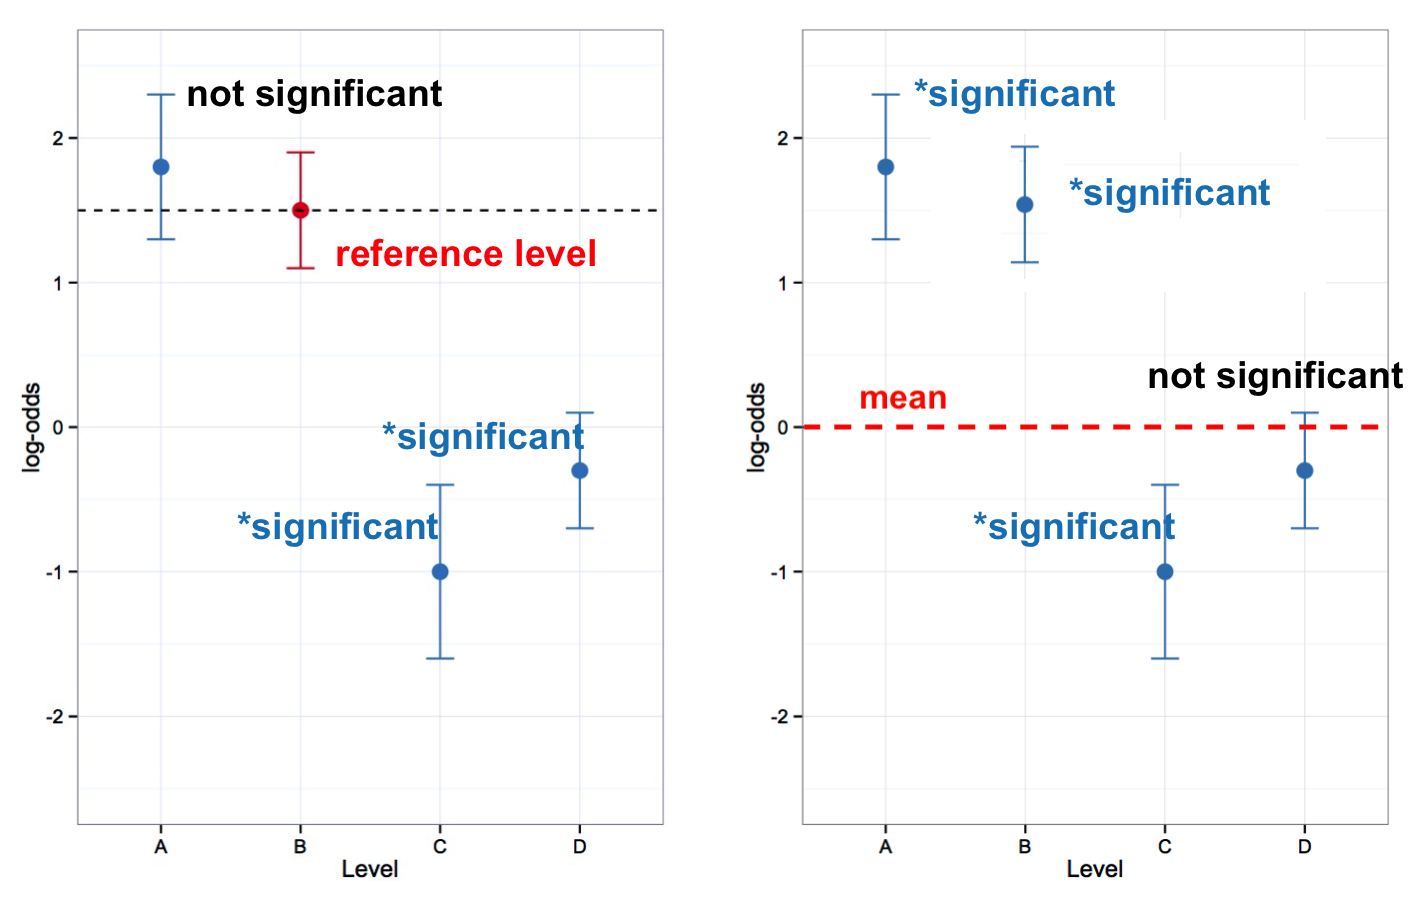
\includegraphics{images/treatmentsum.png}

}

\caption{\label{fig-contrasts}Treatment contrasts (left) versus sum
contrasts (right), ©️ Derek Denis, 2014}

\end{figure}

In
\href{https://lingmethodshub.github.io/content/R/lvc_r/112_lvcr.html}{Part
2} you will do an analyses with sum contrasts, then in
\href{https://lingmethodshub.github.io/content/R/lvc_r/116_lvcr.html}{Part
4} you will do the same analysis, but with treatment contrasts. While
sum contrasts are consistent with a \emph{Goldvarb}-type analysis, you
can probe the constraint hierarchy of your fixed effects using treatment
contrasts in a way not otherwise possible.

\hypertarget{making-your-depandent-variable-binary}{%
\subsection{Making Your Depandent Variable
Binary}\label{making-your-depandent-variable-binary}}

I recommend labelling application value tokens with \texttt{1} and
non-application values as \texttt{0} because \emph{R} eventually does
this behind the scenes anyway. For example, with the \texttt{ctree()}
function
(\href{https://lingmethodshub.github.io/content/R/lvc_r/080_lvcr.html}{Conditional
Inference Trees}) and \texttt{glmer()} function below, the dependent
variable used is \texttt{Dep.Var}. This variable has two levels
\texttt{Realization} and \texttt{Deletion}. Before using these values in
either model, \emph{R} will convert each level to \texttt{0} and
\texttt{1} in alphabetical order. So here \texttt{Deletion} becomes
\texttt{0} and \texttt{Realization} becomes \texttt{1}. This causes
complications for us because, for both \texttt{ctree()} and
\texttt{glmer()}, likelihood is expressed as the likelihood of
\texttt{1}, and \texttt{1} here is the non-application value. You don't
want to use the likelihood of the non-application value in your
manuscript tables and charts! You want to include values in your tables
and charts that reflect the probability of, in this case,
\texttt{0}.\footnote{I also recognize that labelling the application
  value as \texttt{1} can get confusing when the phenomenon in question
  is \texttt{Deletion}. This is the advantage of having two
  \texttt{Dep.Var} columns: one with the dependant variable clearly
  labeled (e.g., \texttt{Deletion} and \texttt{Realized}), and another
  column with the dependent variable in binary format (e.g., \texttt{1}
  and \texttt{0}). Having both ensures you are never confused as to what
  the simplified binary coding means.}

There are two ways to overcome the above problem. You can change the
ordering of the factors in the \texttt{Dep.Var} column so that the
non-application value will be converted to \texttt{0} and the
application value will be converted to \texttt{1}. This is exactly what
was done when constructing the \texttt{ctree()} in
\href{https://lingmethodshub.github.io/content/R/lvc_r/080_lvcr.html}{Conditional
Inference Trees} by changing the order of the levels in \texttt{Dep.Var}
to \texttt{Realized} then \texttt{Deletion} (so \texttt{Realized}
becomes \texttt{0} and \texttt{Deletion} becomes \texttt{1}).
Alternatively, you can create a new column with \texttt{Realization}
tokens coded as \texttt{0} and \texttt{Deletion} tokens coded as
\texttt{1} (see the tip below), then use that new column in your models.
The one disadvantage to this method is that in your figures, like the
\texttt{ctree()} figure created in
\href{https://lingmethodshub.github.io/content/R/lvc_r/080_lvcr.html}{Conditional
Inference Trees}, the names of the two levels of \texttt{Dep.Var} on the
figure itself will be \texttt{1} and \texttt{0}. For the
\texttt{glmer()} function this doesn't really matter.

\begin{tcolorbox}[enhanced jigsaw, colbacktitle=quarto-callout-tip-color!10!white, opacityback=0, left=2mm, breakable, bottomrule=.15mm, colback=white, colframe=quarto-callout-tip-color-frame, toprule=.15mm, arc=.35mm, rightrule=.15mm, toptitle=1mm, opacitybacktitle=0.6, bottomtitle=1mm, coltitle=black, leftrule=.75mm, titlerule=0mm, title=\textcolor{quarto-callout-tip-color}{\faLightbulb}\hspace{0.5em}{Get the data first}]

If you don't have the \texttt{td} data loaded in \emph{R}, go back to
\href{https://lingmethodshub.github.io/content/R/lvc_r/050_lvcr.html}{Doing
it all again, but \texttt{tidy}} and run the code.

\end{tcolorbox}

\begin{Shaded}
\begin{Highlighting}[]
\CommentTok{\# Reorder levels of Dep.Var to make application}
\CommentTok{\# value second}
\NormalTok{td}\SpecialCharTok{$}\NormalTok{Dep.Var }\OtherTok{\textless{}{-}} \FunctionTok{factor}\NormalTok{(td}\SpecialCharTok{$}\NormalTok{Dep.Var, }\AttributeTok{levels =} \FunctionTok{c}\NormalTok{(}\StringTok{"Realized"}\NormalTok{,}
    \StringTok{"Deletion"}\NormalTok{))}
\CommentTok{\# Create New Column for binary Dependent}
\CommentTok{\# Variable, all values 0}
\NormalTok{td}\SpecialCharTok{$}\NormalTok{Dep.Var.Binary }\OtherTok{\textless{}{-}} \StringTok{"0"}
\CommentTok{\# Change all Dep.Var.Binary tokens to 1 where}
\CommentTok{\# Dep.Var.Full is \textquotesingle{}Deletion\textquotesingle{}.}
\NormalTok{td}\SpecialCharTok{$}\NormalTok{Dep.Var.Binary[td}\SpecialCharTok{$}\NormalTok{Dep.Var.Full }\SpecialCharTok{==} \StringTok{"Deletion"}\NormalTok{] }\OtherTok{\textless{}{-}} \StringTok{"1"}
\CommentTok{\# Make Dep.Var.Binary a factor column}
\NormalTok{td}\SpecialCharTok{$}\NormalTok{Dep.Var.Binary }\OtherTok{\textless{}{-}} \FunctionTok{factor}\NormalTok{(td}\SpecialCharTok{$}\NormalTok{Dep.Var.Binary)}
\end{Highlighting}
\end{Shaded}

\begin{tcolorbox}[enhanced jigsaw, colbacktitle=quarto-callout-tip-color!10!white, opacityback=0, left=2mm, breakable, bottomrule=.15mm, colback=white, colframe=quarto-callout-tip-color-frame, toprule=.15mm, arc=.35mm, rightrule=.15mm, toptitle=1mm, opacitybacktitle=0.6, bottomtitle=1mm, coltitle=black, leftrule=.75mm, titlerule=0mm, title=\textcolor{quarto-callout-tip-color}{\faLightbulb}\hspace{0.5em}{A Note on Dependent Variables with 3+ levels}]

Both the \texttt{ctree()} and \texttt{glmer()} functions require binary
dependent variables. If you have a study in which you have a dependent
variable with multiple variants (like the \texttt{Dep.Var.Full} column),
you should make a separate column in which all the tokens with the
application value are labelled as one thing, and all the tokens with any
non-application value are labelled with another (this is effectively
what the \texttt{Dep.Var} column is).

Making this binary column is quite easy in \emph{R}. I like to use the
binary values \texttt{1} and \texttt{0}, with \texttt{1} as my
application value and \texttt{0} as my non-application value. To do this
recode, first you create a new column and make every value \texttt{0}.
Then you change the value in this column to \texttt{1} for every token
where \texttt{Dep.Var.Full} equals the application value. Lastly you
make this column a factor column (though you could use the function
\texttt{as.numeric()} to make a numeric column, if that were needed).

\end{tcolorbox}



\end{document}
